\chapter{Divergence, Cross-Entropy, and Metric Spaces}

\section{The Geometry of Belief}
Machine learning, at its core, is an exercise in approximation. We are granted access to a limited set of observations drawn from an unknown, underlying reality, and we are tasked with constructing a surrogate model that mimics this reality as closely as possible. In the language of probability, we are given samples from a true data distribution $P$, and we seek a model distribution $Q$ that approximates $P$. But what does it mean for two distributions to be ``close''?

In physical space, distance is unambiguous. The distance between two cities can be measured with a ruler and obeys intuitive geometric rules: it is symmetric (the distance from $A$ to $B$ is the distance from $B$ to $A$), and it satisfies the triangle inequality (the detour through $C$ cannot be shorter than the straight line from $A$ to $B$). Spaces equipped with such a distance function are called metric spaces.

However, the space of probability distributions---often termed the statistical manifold---does not naturally yield to the geometry of physical space. When we modify our beliefs or update a model's parameters, we are traversing this space, and the ``distance'' we measure is fundamentally tied to information, not physical length. The cost of replacing the true distribution $P$ with an approximation $Q$ is best understood through the lens of encoding and surprisal.

This brings us to the concept of Cross-Entropy and the Kullback-Leibler (KL) divergence. Cross-entropy measures the total expected cost of encoding events from $P$ using a coding scheme optimized for $Q$. The KL divergence represents the \textit{excess} cost, the penalty incurred precisely because $Q$ is not $P$. Unlike physical distance, information divergence is inherently asymmetric. It is far more penalizing to assign zero probability to an event that actually occurs than to assign positive probability to an event that never occurs. This asymmetry reflects the directional nature of learning and approximation: the model $Q$ must conform to the reality $P$, not the other way around.

As we delve into the mathematical formulations of these concepts, we must abandon our reliance on simple Euclidean intuition. We will see that while KL divergence lacks the properties of a true metric, it provides a profoundly meaningful measure of informational discrepancy. We will also explore how to bridge the gap between information divergence and true metric spaces, paving the way for advanced tools in deep learning.

\section{Mathematical Foundations of Divergence}

To quantify the difference between two probability distributions, we begin with Cross-Entropy.

\begin{definition}[Cross-Entropy]
Let $P$ and $Q$ be two probability distributions defined over the same discrete support $\mathcal{X}$. The cross-entropy $H(P, Q)$ is defined as the expected surprisal of events from $P$ when evaluated under the model $Q$:
\begin{equation}
H(P, Q) = -\sum_{x \in \mathcal{X}} P(x) \log Q(x)
\end{equation}
For continuous distributions with probability density functions $p(x)$ and $q(x)$, the cross-entropy is:
\begin{equation}
H(P, Q) = -\int_{\mathcal{X}} p(x) \log q(x) \, dx
\end{equation}
\end{definition}

Cross-entropy is the standard objective function in classification tasks within deep learning, where $P$ represents the empirical distribution (one-hot labels) and $Q$ is the network's predicted softmax distribution.

The cross-entropy can be decomposed into the entropy of the true distribution $P$ and the Kullback-Leibler divergence from $P$ to $Q$.

\begin{definition}[Kullback-Leibler Divergence]
The Kullback-Leibler (KL) divergence, or relative entropy, from $P$ to $Q$ is defined as:
\begin{equation}
D_{\text{KL}}(P \parallel Q) = \sum_{x \in \mathcal{X}} P(x) \log \frac{P(x)}{Q(x)}
\end{equation}
\end{definition}

\begin{theorem}[Cross-Entropy Decomposition]
For any two distributions $P$ and $Q$ over $\mathcal{X}$,
\begin{equation}
H(P, Q) = H(P) + D_{\text{KL}}(P \parallel Q)
\end{equation}
\end{theorem}
\begin{proof}
By direct substitution of the definitions:
\begin{align*}
H(P, Q) &= -\sum_{x \in \mathcal{X}} P(x) \log Q(x) \\
&= -\sum_{x \in \mathcal{X}} P(x) \log Q(x) + \sum_{x \in \mathcal{X}} P(x) \log P(x) - \sum_{x \in \mathcal{X}} P(x) \log P(x) \\
&= -\sum_{x \in \mathcal{X}} P(x) \log P(x) + \sum_{x \in \mathcal{X}} P(x) \left( \log P(x) - \log Q(x) \right) \\
&= H(P) + \sum_{x \in \mathcal{X}} P(x) \log \frac{P(x)}{Q(x)} \\
&= H(P) + D_{\text{KL}}(P \parallel Q)
\end{align*}
Since $H(P)$ depends solely on the data distribution and is fixed with respect to model parameters, minimizing the cross-entropy $H(P, Q)$ is strictly equivalent to minimizing the KL divergence $D_{\text{KL}}(P \parallel Q)$.
\end{proof}

A foundational property of the KL divergence is that it is non-negative, formalizing the intuition that any approximation $Q$ can only be sub-optimal or perfectly equal to $P$. This is established by Gibbs' Inequality.

\begin{theorem}[Gibbs' Inequality]
For any two probability distributions $P$ and $Q$, $D_{\text{KL}}(P \parallel Q) \ge 0$. Furthermore, $D_{\text{KL}}(P \parallel Q) = 0$ if and only if $P(x) = Q(x)$ for all $x \in \mathcal{X}$ almost everywhere.
\end{theorem}
\begin{proof}
We employ Jensen's Inequality, which states that for any strictly convex function $f$ and non-degenerate random variable $Z$, $\mathbb{E}[f(Z)] \ge f(\mathbb{E}[Z])$. The function $f(t) = -\log(t)$ is strictly convex on $(0, \infty)$.
\begin{align*}
D_{\text{KL}}(P \parallel Q) &= \sum_{x \in \mathcal{X}} P(x) \log \frac{P(x)}{Q(x)} \\
&= \sum_{x \in \mathcal{X}} P(x) \left( -\log \frac{Q(x)}{P(x)} \right) \\
&= \mathbb{E}_{X \sim P}\left[ -\log \frac{Q(X)}{P(X)} \right]
\end{align*}
Applying Jensen's Inequality:
\begin{align*}
\mathbb{E}_{X \sim P}\left[ -\log \frac{Q(X)}{P(X)} \right] &\ge -\log \left( \mathbb{E}_{X \sim P}\left[ \frac{Q(X)}{P(X)} \right] \right) \\
&= -\log \left( \sum_{x \in \mathcal{X}} P(x) \frac{Q(x)}{P(x)} \right) \\
&= -\log \left( \sum_{x \in \mathcal{X}} Q(x) \right)
\end{align*}
Since $Q$ is a valid probability distribution, its sum over the support must be less than or equal to $1$ (equal to $1$ if the support of $Q$ perfectly contains the support of $P$). Thus, $\sum_x Q(x) \le 1$. Since $-\log$ is a monotonically decreasing function, it follows that:
\begin{equation*}
D_{\text{KL}}(P \parallel Q) \ge -\log(1) = 0
\end{equation*}
Because $f(t) = -\log(t)$ is strictly convex, equality holds if and only if the random variable $\frac{Q(X)}{P(X)}$ is a constant with probability $1$. Given that both $P$ and $Q$ integrate to $1$, this constant must be $1$, implying $P(x) = Q(x)$ almost everywhere.
\end{proof}

\begin{figure}[htbp]
\centering
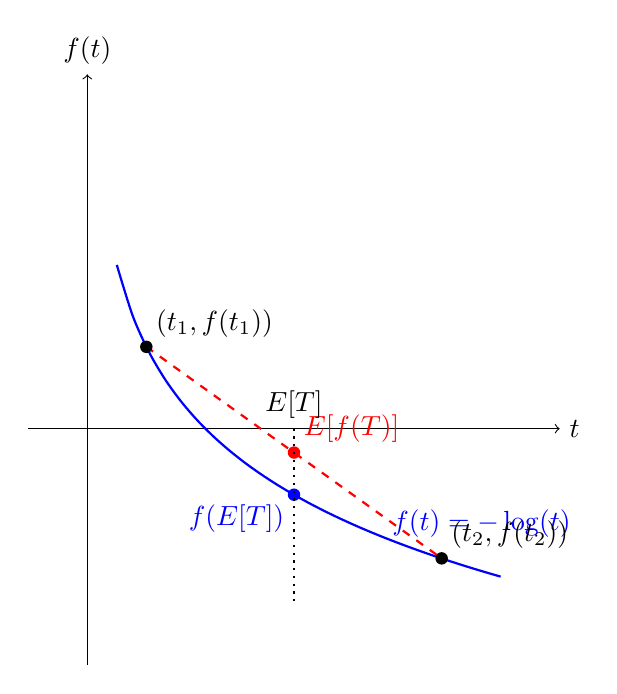
\begin{tikzpicture}[scale=1.5]
  % Draw axes
  \draw[->] (-0.5, 0) -- (4, 0) node[right] {$t$};
  \draw[->] (0, -2) -- (0, 3) node[above] {$f(t)$};
  
  % Draw strictly convex function -log(t)
  \draw[domain=0.25:3.5, smooth, variable=\t, blue, thick] plot ({\t}, {-ln(\t)});
  \node[blue, right] at (2.5, -0.8) {$f(t) = -\log(t)$};
  
  % Draw points and secant line
  \coordinate (A) at (0.5, 0.693);
  \coordinate (B) at (3, -1.098);
  
  \draw[red, dashed, thick] (A) -- (B);
  
  \fill[black] (A) circle (1.5pt) node[above right] {$(t_1, f(t_1))$};
  \fill[black] (B) circle (1.5pt) node[above right] {$(t_2, f(t_2))$};
  
  \coordinate (C) at (1.75, -0.202); % Midpoint on secant line
  \fill[red] (C) circle (1.5pt) node[above right, text=red] {$\mathbb{E}[f(T)]$};
  
  \coordinate (D) at (1.75, -0.559); % Value on function curve
  \fill[blue] (D) circle (1.5pt) node[below left, text=blue] {$f(\mathbb{E}[T])$};
  
  \draw[dotted, thick] (1.75, 0) node[above] {$\mathbb{E}[T]$} -- (1.75, -1.5);
\end{tikzpicture}
\caption{An illustration of Jensen's Inequality for the strictly convex function $f(t) = -\log(t)$. The expected value of the function (evaluated on the red secant line) is strictly greater than or equal to the function of the expected value (on the blue curve). This geometric property is the foundation for proving that $D_{\text{KL}} \ge 0$.}
\label{fig:jensens}
\end{figure}

\subsection{Asymmetry and Mode-Seeking vs. Mean-Seeking Behavior}

The Kullback-Leibler divergence is not a true metric because it is inherently asymmetric: $D_{\text{KL}}(P \parallel Q) \ne D_{\text{KL}}(Q \parallel P)$ in the general case. Furthermore, it does not satisfy the triangle inequality. The choice of direction when minimizing KL divergence profoundly impacts the behavior of the resulting approximation $Q$.

\begin{itemize}
    \item \textbf{Forward KL} ($D_{\text{KL}}(P \parallel Q)$): This is the standard objective in deep learning (equivalent to Maximum Likelihood). The term $P(x) \log \frac{P(x)}{Q(x)}$ implies that if $P(x) > 0$, $Q(x)$ must also be strictly greater than $0$ to avoid an infinite penalty ($\log \frac{P(x)}{0} \to \infty$). Thus, $Q$ is forced to cover all regions where $P$ has mass. When $Q$ is a simpler distribution than $P$, this leads to a \textit{mean-seeking} or \textit{mass-covering} behavior.
    \item \textbf{Reverse KL} ($D_{\text{KL}}(Q \parallel P)$): This formulation is common in Variational Inference (e.g., maximizing the ELBO). Here, the term is $Q(x) \log \frac{Q(x)}{P(x)}$. If $P(x) = 0$, $Q(x)$ must be exactly $0$ to avoid an infinite penalty. The model $Q$ will strongly tend to place mass only where $P$ has high mass, aggressively avoiding regions where $P$ is low. This leads to \textit{mode-seeking} behavior, where $Q$ often captures a single mode of a multimodal $P$, heavily underestimating the true variance.
\end{itemize}

\begin{figure}[htbp]
\centering
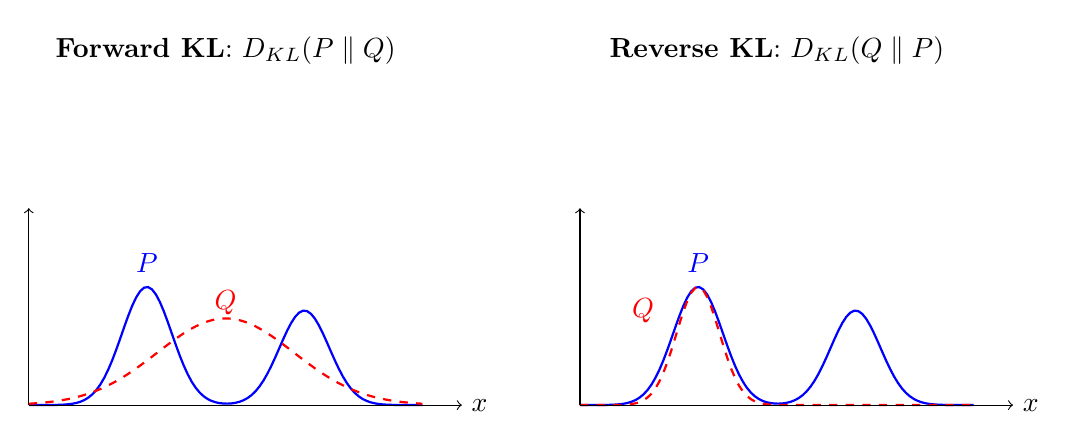
\begin{tikzpicture}[scale=1]
  % Forward KL (Mean-Seeking)
  \begin{scope}[xshift=0cm]
    \node at (2.5, 4.5) {\textbf{Forward KL}: $D_{\text{KL}}(P \parallel Q)$};
    % P(x) bimodal
    \draw[blue, thick, domain=0:5, samples=100] plot (\x, {1.5*exp(-(\x-1.5)^2/0.2) + 1.2*exp(-(\x-3.5)^2/0.2)});
    \node[blue] at (1.5, 1.8) {$P$};
    % Q(x) unimodal covering both
    \draw[red, dashed, thick, domain=0:5, samples=100] plot (\x, {1.1*exp(-(\x-2.5)^2/1.5)});
    \node[red] at (2.5, 1.3) {$Q$};
    \draw[->] (0,0) -- (5.5,0) node[right] {$x$};
    \draw[->] (0,0) -- (0,2.5);
  \end{scope}
  
  % Reverse KL (Mode-Seeking)
  \begin{scope}[xshift=7cm]
    \node at (2.5, 4.5) {\textbf{Reverse KL}: $D_{\text{KL}}(Q \parallel P)$};
    % P(x) bimodal
    \draw[blue, thick, domain=0:5, samples=100] plot (\x, {1.5*exp(-(\x-1.5)^2/0.2) + 1.2*exp(-(\x-3.5)^2/0.2)});
    \node[blue] at (1.5, 1.8) {$P$};
    % Q(x) unimodal capturing one mode
    \draw[red, dashed, thick, domain=0:5, samples=100] plot (\x, {1.5*exp(-(\x-1.5)^2/0.15)});
    \node[red] at (0.8, 1.2) {$Q$};
    \draw[->] (0,0) -- (5.5,0) node[right] {$x$};
    \draw[->] (0,0) -- (0,2.5);
  \end{scope}
\end{tikzpicture}
\caption{The geometric asymmetry of the Kullback-Leibler Divergence. Forward KL penalizes failing to cover mass, forcing the approximation $Q$ (red dashed) to bridge the modes of the target $P$ (blue solid). Reverse KL penalizes placing mass where the target has none, encouraging $Q$ to tightly fit a single mode of $P$.}
\label{fig:kl_asymmetry}
\end{figure}

\subsection{Numerical Example: Evaluating Divergence}
Let us consider a discrete binary event, such as a coin toss, to explicitly compute these quantities. Suppose the true distribution $P$ of a biased coin is $P(\text{Heads}) = 0.8, P(\text{Tails}) = 0.2$. We propose two distinct candidate models:
\begin{itemize}
    \item $Q_1$: A closely matching model with $Q_1(\text{Heads}) = 0.9, Q_1(\text{Tails}) = 0.1$.
    \item $Q_2$: A naive uniform model with $Q_2(\text{Heads}) = 0.5, Q_2(\text{Tails}) = 0.5$.
\end{itemize}
We calculate the Forward KL divergence in nats (using the natural logarithm):
\begin{align*}
D_{\text{KL}}(P \parallel Q_1) &= 0.8 \ln\left(\frac{0.8}{0.9}\right) + 0.2 \ln\left(\frac{0.2}{0.1}\right) \\
&\approx 0.8 \times (-0.1178) + 0.2 \times (0.6931) \approx 0.0444 \text{ nats}
\end{align*}
\begin{align*}
D_{\text{KL}}(P \parallel Q_2) &= 0.8 \ln\left(\frac{0.8}{0.5}\right) + 0.2 \ln\left(\frac{0.2}{0.5}\right) \\
&\approx 0.8 \times (0.4700) + 0.2 \times (-0.9163) \approx 0.1927 \text{ nats}
\end{align*}
As expected, $Q_1$ yields a much lower KL penalty, indicating it is information-theoretically ``closer'' to $P$ than the uniform distribution $Q_2$. Furthermore, we can compute the Reverse KL for $Q_1$:
\begin{align*}
D_{\text{KL}}(Q_1 \parallel P) &= 0.9 \ln\left(\frac{0.9}{0.8}\right) + 0.1 \ln\left(\frac{0.1}{0.2}\right) \\
&\approx 0.9 \times (0.1178) + 0.1 \times (-0.6931) \approx 0.0367 \text{ nats}
\end{align*}
Notice that $0.0367 \text{ nats} \ne 0.0444 \text{ nats}$, which numerically confirms the fundamental asymmetry of the divergence.

\subsection{From Divergence to Metric Spaces: Pinsker's Inequality}

While KL divergence is not a metric, it provides strict bounds on true metric distances operating on the statistical manifold. The most prominent example is the Total Variation (TV) distance, a true metric that evaluates the largest possible difference in probability assigned to any single event.

\begin{definition}[Total Variation Distance]
The Total Variation distance $\delta(P, Q)$ between two probability distributions $P$ and $Q$ on a sample space $\mathcal{X}$ is defined as:
\begin{equation}
\delta(P, Q) = \sup_{A \subseteq \mathcal{X}} |P(A) - Q(A)| = \frac{1}{2}\sum_{x \in \mathcal{X}} |P(x) - Q(x)|
\end{equation}
\end{definition}

Unlike divergence, TV distance satisfies symmetry and the triangle inequality. Pinsker's Inequality provides a foundational bridge, demonstrating that convergence in information divergence forces convergence in the $L_1$ metric geometry.

\begin{theorem}[Pinsker's Inequality]
For any two distributions $P$ and $Q$,
\begin{equation}
\delta(P, Q) \le \sqrt{\frac{1}{2} D_{\text{KL}}(P \parallel Q)}
\end{equation}
\end{theorem}
This inequality is critical for deep learning guarantees. If an optimization procedure drives the cross-entropy down to the true entropy $H(P)$---meaning the KL divergence is driven to zero---Pinsker's inequality guarantees that the model's predictions pointwise converge to the true probabilities in a rigorous metric sense.

\begin{horizon}
The mathematical necessity of asymmetric divergences like KL has dominated the last decade of deep learning, largely due to the sheer tractability of maximum likelihood estimation. However, it is deeply conjectured that the strict reliance on KL divergence is a computational compromise rather than an architectural ideal. An open question is whether the future of generative modeling lies entirely in true metric spaces, such as Wasserstein distances parameterized by Optimal Transport theory, which elegantly handle disjoint distributions where KL divergence approaches infinity and gradients vanish.

Furthermore, some theorists conjecture that standard gradient descent on the cross-entropy loss implicitly approximates a natural gradient flow over the statistical manifold. This suggests that modern optimizers might be navigating metric constraints that are not explicitly coded into the objective function. Future work might show that heavily parameterized networks naturally regularize their own trajectories in weight space to mimic optimal transport on the probability simplex, effectively blurring the boundary between the $f$-divergences we optimize and the true metric spaces we intend to traverse. If this implicit geometry can be formalized, it would profoundly shift our understanding of why deep neural networks generalize reliably despite minimizing purely pointwise informational bounds.
\end{horizon}

\section{Summary}
In this chapter, we explored the geometric and information-theoretic interpretation of distribution approximation. We formalized Cross-Entropy and decomposed it into the irreducible entropy of the data and the Kullback-Leibler divergence. Through Gibbs' Inequality, we proved that KL divergence acts as a non-negative discrepancy measure. We examined its fundamental asymmetry---revealing the distinct mode-seeking and mean-seeking behaviors of Reverse and Forward KL respectively---and demonstrated via Pinsker's Inequality how purely informational divergences serve as strict bounds on true $L_1$ metric spaces like the Total Variation distance.

\section{Exercises}
\begin{enumerate}
    \item \textbf{Non-negativity of Cross-Entropy:} Prove that if $P$ and $Q$ are discrete probability distributions, the cross-entropy $H(P, Q)$ is strictly bounded below by the Shannon entropy $H(P)$. Under what condition is $H(P, Q) = H(P)$?
    \item \textbf{Symmetry Failure:} Construct two discrete distributions $P$ and $Q$ over a three-element set $\{a, b, c\}$ such that $D_{\text{KL}}(P \parallel Q)$ is more than twice $D_{\text{KL}}(Q \parallel P)$.
    \item \textbf{Continuous KL Divergence:} Given two univariate Gaussian distributions $P = \mathcal{N}(\mu_1, \sigma_1^2)$ and $Q = \mathcal{N}(\mu_2, \sigma_2^2)$, derive the closed-form expression for $D_{\text{KL}}(P \parallel Q)$. Show analytically that this divergence is symmetric if and only if $\sigma_1 = \sigma_2$.
    \item \textbf{Pinsker's Bound in Practice:} Using the coin toss distributions from the numerical example ($P(\text{Heads})=0.8, Q_1(\text{Heads})=0.9$), calculate the exact Total Variation distance $\delta(P, Q_1)$ and explicitly verify that the bound given by Pinsker's Inequality holds.
\end{enumerate}

% TODO-CITE: Ensure all named results are cited.
